%Docmment Class
\documentclass[12pt,report]{article}

%Packages
\usepackage{titlesec}
\usepackage{blindtext}
\usepackage{microtype}
\usepackage{booktabs}
\usepackage{placeins}
\usepackage{enumitem}
\usepackage{xcolor}
\usepackage{xhfill}
\usepackage{multicol}
\usepackage{float}
\usepackage{url}
\usepackage[hidelinks]{hyperref}
\usepackage[margin=0.5in]{geometry}
\usepackage{graphicx}
\usepackage{tikz}

%Formating for Control Logic Process Diagram
\tikzstyle{start} = [rectangle, rounded corners, text width = 15cm, minimum height=1cm, text centered, draw=black, fill=purple!60]
\tikzstyle{stop} = [rectangle, rounded corners, text width = 15cm, minimum height=1cm, text centered, draw=black, fill=purple!60]
\tikzstyle{process} = [rectangle,text width = 19cm, minimum height=1cm, text centered, draw=black, fill=purple!40]
\tikzstyle{arrow} = [thick,->,>-stealth]

%Section Formatting
%\titlespacing{\section}{0pt}{*1}{*1}

\titleformat{\section}
    {\LARGE\bfseries}{\filright\footnotesize\enspace SECTION\thesection\enspace}{12pt}
    {\titlerule[1.6pt]}

\titleformat{\subsection}
    {\large\bfseries}{\thesection}{1em}{}
    % [{\titlerule[0.8pt]}]

\setlength{\parindent}{0pt}%

\pagenumbering{gobble}
\date{}

\begin{document}

\section*{Github - Procedures}

The purpose of this document is provide guidance for common github commands so we can efficiently commit changes from the command line.

\subsection*{Creating Local Repository and Connecting to Remote Repository}

\begin{figure}[H]
	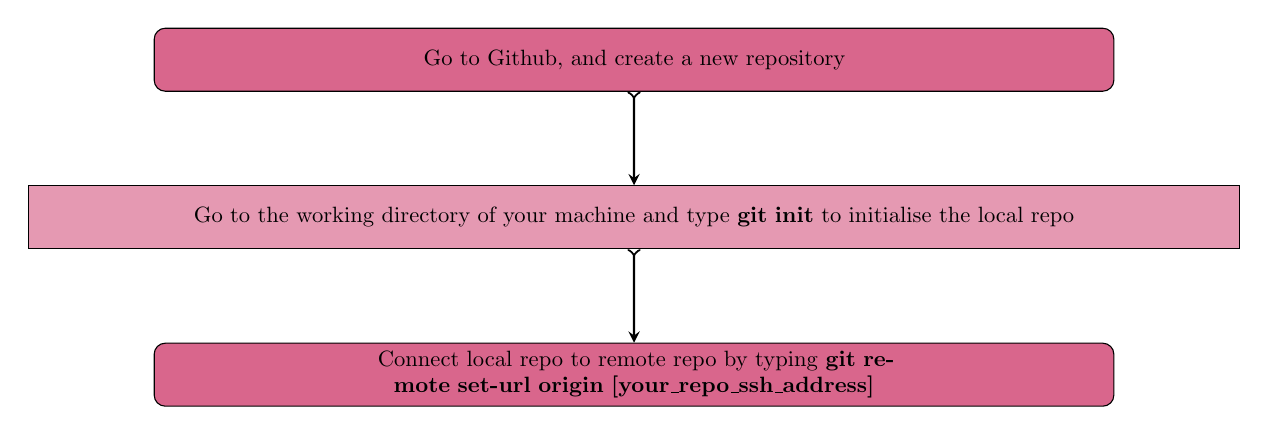
\begin{tikzpicture}[node distance = 2.5cm,every node/.style={scale=0.8}]

	\node (start) [start] {Go to Github, and create a new repository};
		\node (init) [process,below of=start] {Go to the working directory of your machine and type \textbf{git init} to initialise the local repo};
		\node (remote) [stop,below of=init] {Connect local repo to remote repo by typing \textbf{git remote set-url origin [your\_repo\_ssh\_address]}};

	\draw [arrow] (start) -- (init){};
	\draw [arrow] (init) -- (remote) {};

\end{tikzpicture}
\centering
\end{figure}

\subsection*{Cloning a Github Repository}

\begin{figure}[H]
	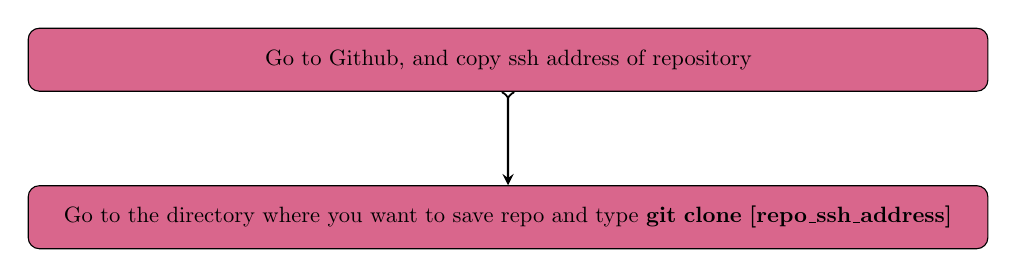
\begin{tikzpicture}[node distance = 2.5cm,every node/.style={scale=0.8}]

	\node (start) [start] {Go to Github, and copy ssh address of repository};
		\node (init) [stop,below of=start] {Go to the directory where you want to save repo and type \textbf{git clone [repo\_ssh\_address]}};

	\draw [arrow] (start) -- (init){};

\end{tikzpicture}
\centering
\end{figure}


\subsection*{Creating SSH Keys for Authentication Protocol}

\begin{figure}[H]
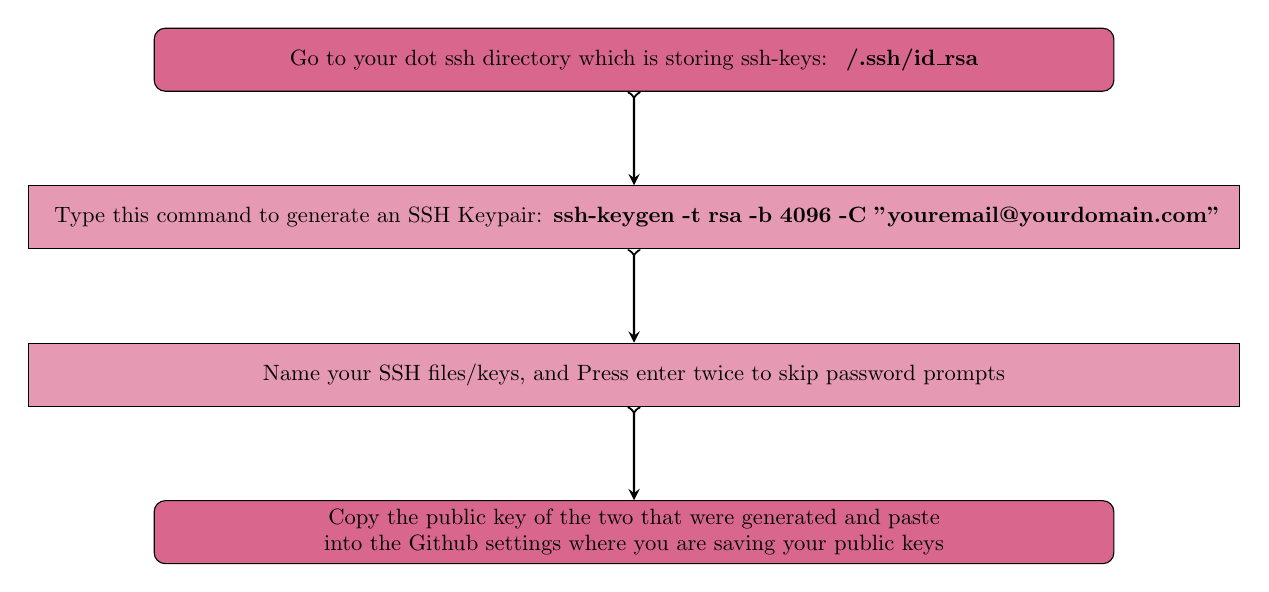
\begin{tikzpicture}[node distance = 2.5cm,every node/.style={scale=0.8}]

	\node (start) [start] {Go to your dot ssh directory which is storing ssh-keys:\textbf{ \url{~}/.ssh/id\_rsa}};
	\node (keygen) [process,below of=start] {Type this command to generate an SSH Keypair: \textbf{ssh-keygen -t rsa -b 4096 -C "youremail@yourdomain.com"}};
	\node (skip) [process,below of=keygen] {Name your SSH files/keys, and Press enter twice to skip password prompts};
	\node (pub) [stop,below of=skip] {Copy the public key of the two that were generated and paste into the Github settings where you are saving your public keys};

	\draw [arrow] (start) -- (keygen){};
	\draw [arrow] (keygen) -- (skip) {};
	\draw [arrow] (skip) -- (pub) {};

\end{tikzpicture}
\centering
\end{figure}

\newpage

\subsection*{Initialise SSH-Agent and Add Private SSH Key To Key Chain}


This process can also be automated using shell scripts or adding the shell commands to a config file to ensure ssh-agent process is initialised and the relevant key is pathed into the keychain.

\begin{figure}[H]
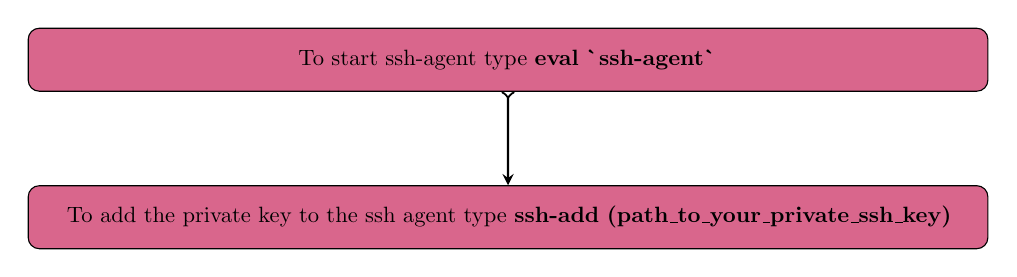
\begin{tikzpicture}[node distance = 2.5cm,every node/.style={scale=0.8}]

	\node (start) [start] {To start ssh-agent type \textbf{eval \`{}ssh-agent\`}};
	\node (ssh-add) [stop,below of=start] {To add the private key to the ssh agent type \textbf{ssh-add (path\_to\_your\_private\_ssh\_key)}};

	\draw [arrow] (start) -- (ssh-add){};

\end{tikzpicture}
\centering
\end{figure}

\subsection*{Commit Changes to Github Repository}


\begin{figure}[H]
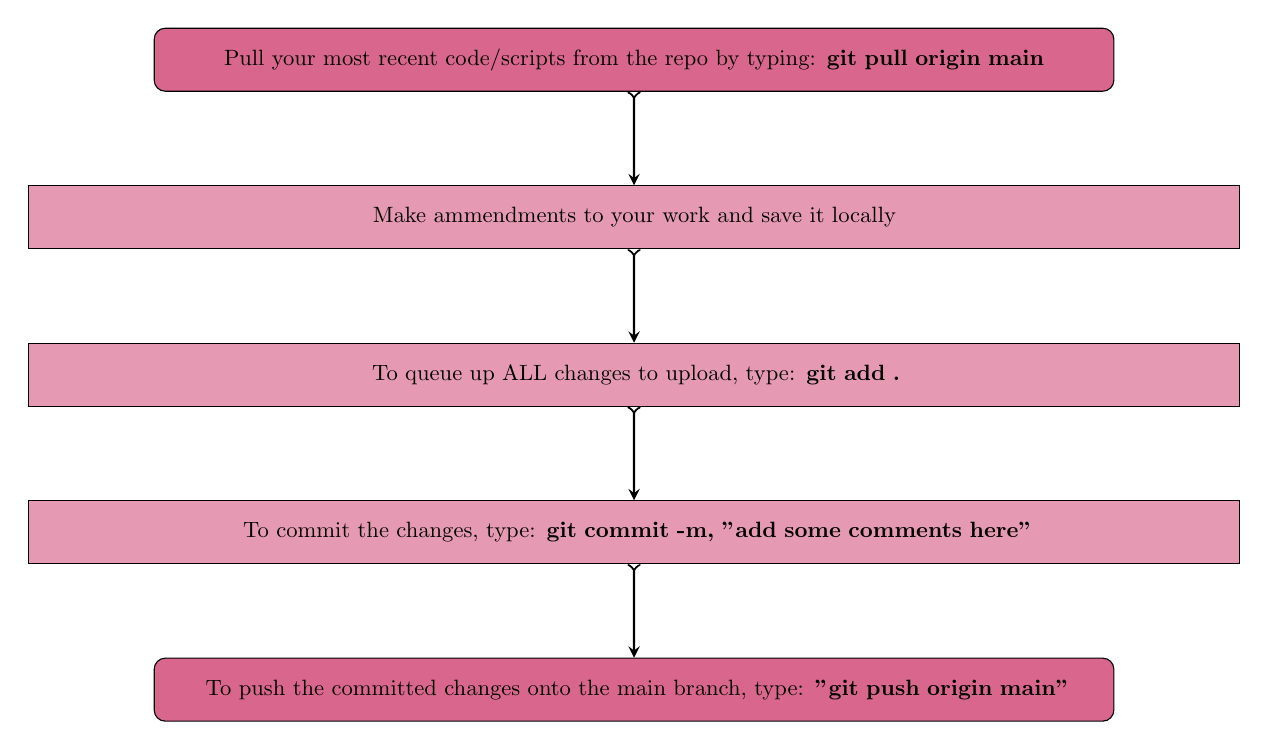
\begin{tikzpicture}[node distance = 2.5cm,every node/.style={scale=0.8}]

	\node (start) [start] {Pull your most recent code/scripts from the repo by typing: \textbf{git pull origin main}};
	\node (work) [process,below of=start] {Make ammendments to your work and save it locally};
	\node (add) [process,below of=work] {To queue up ALL changes to upload, type: \textbf{git add .}};
	\node (commit) [process,below of=add] {To commit the changes, type: \textbf{git commit -m, "add some comments here"}};
	\node (push) [stop,below of=commit] {To push the committed changes onto the main branch, type: \textbf{"git push origin main"}};

	\draw [arrow] (start) -- (work){};
	\draw [arrow] (work) -- (add){};
	\draw [arrow] (add) -- (commit){};
	\draw [arrow] (commit) -- (push){};


\end{tikzpicture}
\centering
\end{figure}


\end{document}\\
